\documentclass[12pt,letterpaper]{article}
\usepackage{natbib}

%Packages
% \usepackage{textcomp}
% \usepackage{latexsym}
% \usepackage{url}
% \usepackage{amssymb}
% \usepackage{amsmath}
% \usepackage{mathtools}
% \usepackage{bm}
% \usepackage{array}
% \usepackage[version=3]{mhchem}
% \usepackage{ifthen}
% \usepackage{amsthm}
% \usepackage{amstext}
% \usepackage{enumerate}
% \usepackage{dcolumn}

\usepackage{epsfig}
\usepackage{graphicx}
\usepackage{caption}
\usepackage{hyperref}
\usepackage{lineno}
\usepackage{pdflscape}
\usepackage{mathtools}
\usepackage[osf]{mathpazo}
\usepackage{fullpage}
\usepackage{float}
\usepackage{xr} %linking to supplementaries
\externaldocument{supplementaries}

\pagenumbering{arabic}


%---------------------------------------------
%
%       START
%
%---------------------------------------------

\begin{document}
%Running head
\begin{flushright}
Version dated: \today
\end{flushright}

\bigskip
\bigskip
\begin{center}

\noindent{\Large \bf The what, how and why of trait-based analyses in ecology}
\bigskip

\noindent {\normalsize \sc
Thomas Guillerme$^{1,*}$, 
Pedro Cardoso$^{2,3}$,
% Carlos P. Carmona$^{4}$,
Maria Wagner J\o rgensen$^{4}$,
Stefano Mammola$^{3,5,6}$,
Thomas J. Matthews$^{4,7}$}\\
\noindent {\small \it 
$^1$School of Biosciences, The University of Sheffield, Sheffield, S10 2TN, United Kingdom.\\
$^2$CE3C—Centre for Ecology, Evolution and Environmental Changes, CHANGE – Global Change and Sustainability Institute, Faculty of Sciences, University of Lisbon, Lisbon, Portugal\\
$^3$Laboratory for Integrative Biodiversity Research (LIBRe), Finnish Museum of Natural History (Luomus), University of Helsinki, Helsinki, Finland\\
% $^4$Institute of Ecology and Earth Sciences, University of Tartu, Tartu, Estonia\\
$^4$School of Geography, Earth and Environmental Sciences and Birmingham Institute of Forest Research, University of Birmingham, Birmingham B15 2TT, UK\\
$^5$Molecular Ecology Group (MEG), Water Research Institute, National Research Council (CNR-IRSA), Verbania Pallanza, Italy\\
$^6$National Biodiversity Future Center, Piazza Marina 61, 90133 Palermo, Italy\\
$^7$Centre for Ecology, Evolution and Environmental Changes/Azorean Biodiversity Group / CHANGE – Global Change and Sustainability Institute and Universidade dos Açores – Faculty of Agricultural Sciences and Environment; PT-9700-042, Angra do Hero\'ismo, A\c ores, Portugal.\\}

\end{center}
\bigskip
\noindent{*\bf Corresponding author.} \textit{t.guillerme@sheffield.ac.uk}\\ 
\vspace{1in}

%Line numbering
\modulolinenumbers[1]
\linenumbers

%---------------------------------------------
%
%       ABSTRACT
%
%---------------------------------------------


\section{Supplementary materials}

\subsection{Glossary}


\begin{table}[ht]
\caption{Glossary and equivalence of terms used in this papers; adapted from \cite{guillerme2018disprity} and \cite{mammola2021concepts}.}
\centering
\begin{tabular}{p{2.5cm}p{4cm}p{5cm}p{5cm}}
Term in this paper & definition & in ecology & in macroevolution \\
\hline
Trait space & Matrix ($n \times d$) with a structural relation between rows and columns & Functional space, morphospace , etc. & Morphospace, traitspace, etc.  \\
\hline
Observations & Rows ($n$) & Taxa, field sites, environments, etc. & Taxa, specimen, populations, elements, OTUs etc. \\
\hline
Dimensions & Columns ($d$) & Traits, Ordination scores, distances, etc. & Traits, ordination scores, distances, etc. \\
\hline
Traits & Columns subset ($b \times n$; $b \leq d$) & uni/multidimensional trait; e.g. geographical location & uni/multidimensional trait; e.g. landmark coordinates \\
\hline
Group & Rows subset ($m \times d$; $m \leq n$) & Treatments, phylogenetic group (clade), etc. & Clades, geological stratum, etc. \\
\hline
Metric & Statistic (i.e. a measure) & Dissimilarity index or metric, hypervolume, functional diversity, etc. & Disparity metric or index \\
\hline
Stressors & An algorithm removing a proportion of the observations & Introduction of invasive species, change of landscape use, climate change, pollution, experimental design, etc. & Mass extinction, Tectonic change, climate change, etc. \\
\hline
Stressors' intensity & The amount of observation removed (percentages) & Proportion of species affected, proportion of temperature change, etc. & Severity of mass extinction,  etc. \\
\end{tabular}
\end{table}



\subsection{Supplementary results}


\begin{figure}[!htbp]
\centering
   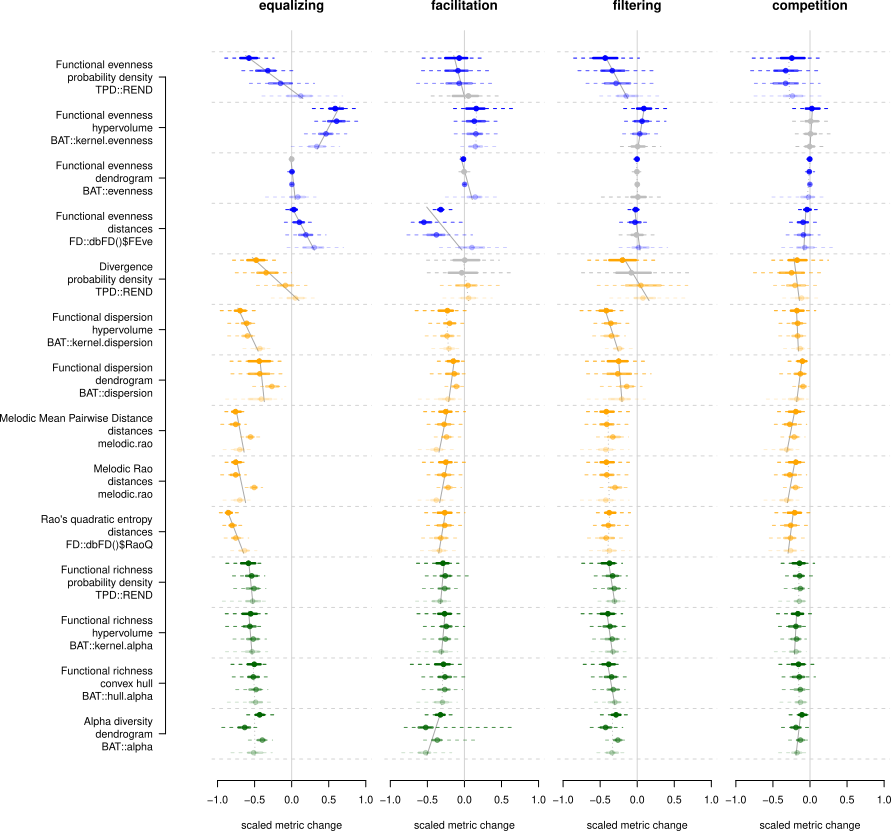
\includegraphics[width=0.8\textwidth]{Figures/results_per_metric_per_stressor_2d.pdf}
\caption{\scriptsize{\textbf{Simulation results for 2 dimensions:} the y axes represent the different metrics tested (sorted by categories).
The different columns represent the different stressors. The x-axes represent the metric values centred on the random changes and scaled by the maximum value for each metric between the four stressors.
Negative and positive values signify that the metric score for the stressor of interest is lower/higher than the one from the random stressor.
The dots represent the median metric value, the full line their 50\% confidence interval (CI) and the dashed line their 95\% CI.
The colours are here to visually separate the metrics by categories (blue = regularity, yellow = divergence, green = richness); the colour gradient within each row corresponds to a removal of respectively 80\%, 60\%, 40\% and 20\% of the data (from top to bottom).
The grey line plots represent distributions of metric scores not clearly distinguishable from the random metric scores (paired t-test p value $> 0.05$).
Grey lines in the background across the distributions of different removal amounts represent the fitted linear model centred and scaled metric score $\sim$ amount of data removed and the value displayed is the adjusted $R^2$ from each of these models.
Dashed thin grey lines represent non-significant models (p value of slope or/and intercept $> 0.05$).
}}
\label{Fig:simulation_results_2d}
\end{figure}
\bigskip


\begin{figure}[!htbp]
\centering
   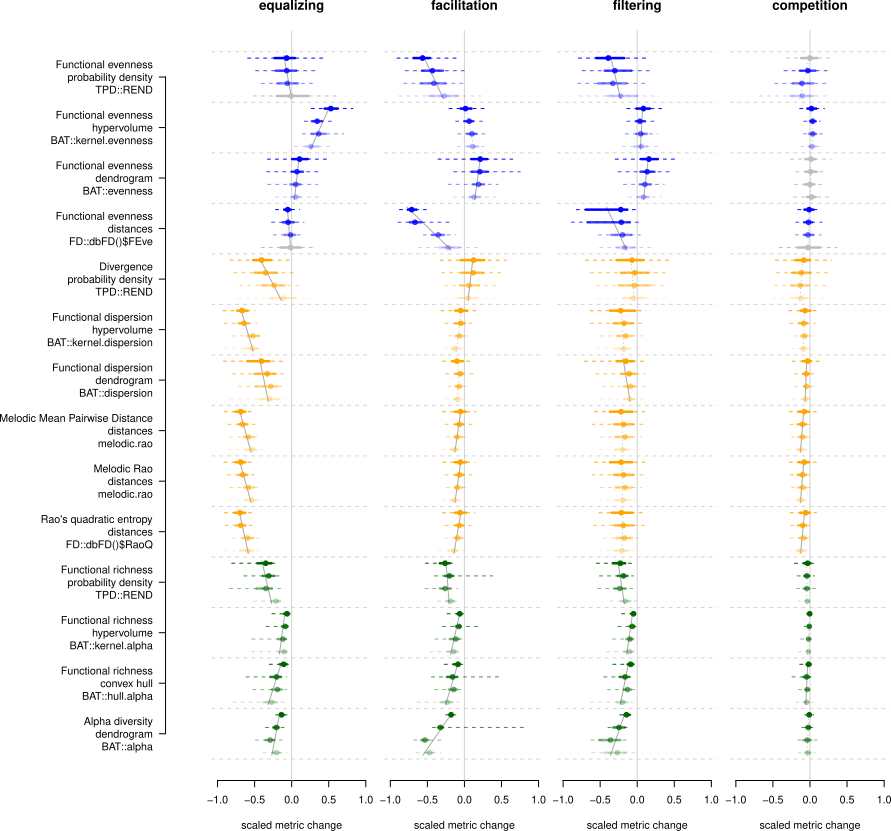
\includegraphics[width=0.8\textwidth]{Figures/results_per_metric_per_stressor_8d.pdf}
\caption{\scriptsize{\textbf{Simulation results for 8 dimensions:} the y axes represent the different metrics tested (sorted by categories).
The different columns represent the different stressors. The x-axes represent the metric values centred on the random changes and scaled by the maximum value for each metric between the four stressors.
Negative and positive values signify that the metric score for the stressor of interest is lower/higher than the one from the random stressor.
The dots represent the median metric value, the full line their 50\% confidence interval (CI) and the dashed line their 95\% CI.
The colours are here to visually separate the metrics by categories (blue = regularity, yellow = divergence, green = richness); the colour gradient within each row corresponds to a removal of respectively 80\%, 60\%, 40\% and 20\% of the data (from top to bottom).
The grey line plots represent distributions of metric scores not clearly distinguishable from the random metric scores (paired t-test p value $> 0.05$).
Grey lines in the background across the distributions of different removal amounts represent the fitted linear model centred and scaled metric score $\sim$ amount of data removed and the value displayed is the adjusted $R^2$ from each of these models.
Dashed thin grey lines represent non-significant models (p value of slope or/and intercept $> 0.05$).
\textbf{NOTE: for the \texttt{TPD} metrics, the metric is calculated using the 4 first dimensions only.}
}}
\label{Fig:simulation_results_8d}
\end{figure}
\bigskip





\begin{figure}[!htbp]
\centering
   \includegraphics[width=0.8\textwidth]{Figures/raw_results_per_metric_per_stressor_2d.pdf}
\caption{\scriptsize{\textbf{Raw metric scores for 2 dimensions:} the y axes represent the different metrics tested (sorted by categories).
The different columns represent the different stressors.
The x-axes represent the scaled metric scores.
The dots represent the median metric value, the full line their 50\% confidence interval (CI) and the dashed line their 95\% CI.
The colours are here to visually separate the metrics by categories (blue = regularity, yellow = divergence, green = richness); the colour gradient within each row corresponds to a removal of respectively 80\%, 60\%, 40\% and 20\% of the data (from top to bottom).
}}
\label{Fig:raw_results_2d}
\end{figure}
\bigskip


\begin{figure}[!htbp]
\centering
   \includegraphics[width=0.8\textwidth]{Figures/raw_results_per_metric_per_stressor_4d.pdf}
\caption{\scriptsize{\textbf{Raw metric scores for 4 dimensions:} the y axes represent the different metrics tested (sorted by categories).
The different columns represent the different stressors.
The x-axes represent the scaled metric scores.
The dots represent the median metric value, the full line their 50\% confidence interval (CI) and the dashed line their 95\% CI.
The colours are here to visually separate the metrics by categories (blue = regularity, yellow = divergence, green = richness); the colour gradient within each row corresponds to a removal of respectively 80\%, 60\%, 40\% and 20\% of the data (from top to bottom).
}}
\label{Fig:raw_results_4d}
\end{figure}
\bigskip


\begin{figure}[!htbp]
\centering
   \includegraphics[width=0.8\textwidth]{Figures/raw_results_per_metric_per_stressor_2d.pdf}
\caption{\scriptsize{\textbf{Raw metric scores for 8 dimensions:} the y axes represent the different metrics tested (sorted by categories).
The different columns represent the different stressors.
The x-axes represent the scaled metric scores.
The dots represent the median metric value, the full line their 50\% confidence interval (CI) and the dashed line their 95\% CI.
The colours are here to visually separate the metrics by categories (blue = regularity, yellow = divergence, green = richness); the colour gradient within each row corresponds to a removal of respectively 80\%, 60\%, 40\% and 20\% of the data (from top to bottom).
}
\textbf{NOTE: for the \texttt{TPD} metrics, the metric is calculated using the 4 first dimensions only.}
}
\label{Fig:raw_results_8d}
\end{figure}
\bigskip


\begin{figure}[!htbp]
\centering
   \includegraphics[width=0.6\textwidth]{Figures/raw_results_per_metric_per_stressor_emp.pdf}
\caption{\scriptsize{\textbf{Raw metric scores for the empirical data:} the y axes represent the different metrics tested (sorted by categories).
The different columns represent the different stressors.
The x-axes represent the scaled metric scores.
The dots represent the median metric value, the full line their 50\% confidence interval (CI) and the dashed line their 95\% CI.
The colours are here to visually separate the metrics by categories (blue = regularity, yellow = divergence, green = richness); the colour gradient within each row corresponds to a removal of respectively 80\%, 60\%, 40\% and 20\% of the data (from top to bottom).
\textbf{NOTE: for the \texttt{TPD} metrics, the metric is calculated using the 4 first dimensions only.}
}}
\label{Fig:raw_results_emp}
\end{figure}
\bigskip




\begin{figure}[!htbp]
\centering
   \includegraphics{Figures/empirical_data_dimensions.pdf}
\caption{\scriptsize{\textbf{Selection of the number of dimensions for the empirical data:} each histograms corresponds to the variance per dimension (dark grey) and the cumulative variance per dimension (light grey) for each group in the empirical data: the 37 currently endemic Hawaiian species (extant species) the 63 species present before 1500 (pre-1500 group). The plot shows that although 4 dimensions are enough to describe at least 95\% of the variance for the extant group, 5 dimensions are required for the pre-1500 group (following the method proposed in \cite{guillerme2023innovation}).
}}
\label{Fig:empirical_dimensions}
\end{figure}
\bigskip










\begin{figure}[!htbp]
\centering
   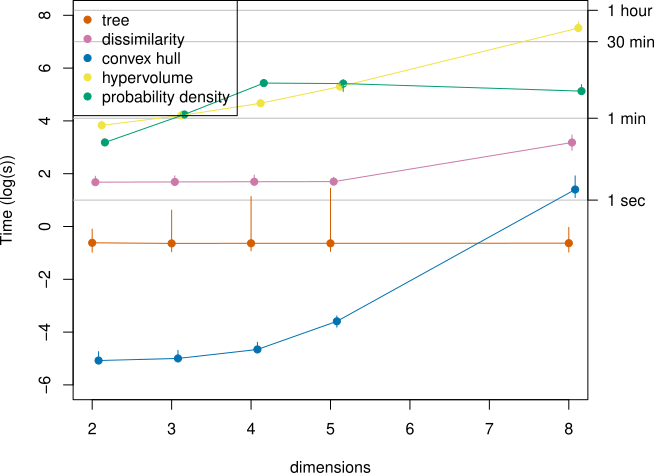
\includegraphics[width=0.8\textwidth]{Figures/time_per_metric}
\caption{\scriptsize{\textbf{Computational time per metric:} log time (seconds) distribution per metric. The dots correspond to the median computational time for one metric for $n$ elements (40, 80, 120, 160) for $D$ dimensions (2, 3, 4, 5, 8). And colour vertical lines represent the 95\% distribution range for each measurement. Note that for the probability density metrics (\texttt{TPD} package), the number of dimensions is restricted to 4. The horizontal grey lines are indicating the log seconds time equivalent in other units (seconds, minutes, hours) for facilitating interpretation.
}}
\label{Fig:metrics_time}
\end{figure}
\bigskip




\begin{landscape}
\begin{table}
\scriptsize
\caption{Results of the model scaled metric $\sim$ removal level per stressor (2D)}
\centering
\begin{tabular}[t]{l|c|c|c|c|c|c|c|c}
\hline
  & equalizing slope & equalizing adj.$R^{2}$ & facilitation slope & facilitation adj.$R^{2}$ & filtering slope & filtering adj.$R^{2}$ & competition slope & competition adj.$R^{2}$\\
\hline
Functional evenness\\distances\\ \texttt{FD::dbFD()\$FEve} & 0.017*** & 0.02 & -0.015** & 0.012 & 0.026*** & 0.057 & -0.001 & -0.001\\
\hline
Functional evenness\\dendrogram\\ \texttt{BAT::evenness} & 0.014** & 0.011 & -0.016** & 0.014 & 0.024*** & 0.038 & -0.009* & 0.007\\
\hline
Functional evenness\\hypervolume\\ \texttt{BAT::kernel.evenness} & 0.007 & 0.002 & -0.006 & 0 & 0.03*** & 0.069 & 0.004 & 0\\
\hline
Functional evenness\\probability density\\ \texttt{TPD::REND} & 0.002 & -0.001 & -0.055*** & 0.07 & 0.001 & -0.001 & -0.02*** & 0.048\\
\hline
Rao's quadratic entropy\\distances\\ \texttt{FD::dbFD()\$RaoQ} & 0.185*** & 0.578 & 0.022** & 0.009 & 0.102*** & 0.117 & 0.022** & 0.013\\
\hline
Functional dispersion\\dendrogram\\ \texttt{BAT::dispersion} & 0.08*** & 0.396 & 0.009. & 0.003 & 0.054*** & 0.195 & 0.008* & 0.005\\
\hline
Functional dispersion\\hypervolume\\ \texttt{BAT::kernel.dispersion} & 0.018** & 0.009 & -0.023*** & 0.04 & 0.014* & 0.004 & -0.022*** & 0.048\\
\hline
Divergence\\probability density\\ \texttt{TPD::REND} & 0.066*** & 0.436 & -0.028*** & 0.046 & -0.009. & 0.004 & -0.022*** & 0.038\\
\hline
Alpha diversity\\dendrogram\\ \texttt{BAT::alpha} & 0.227*** & 0.572 & 0.044*** & 0.037 & 0.091*** & 0.155 & 0.002 & -0.001\\
\hline
Functional richness\\convex hull\\ \texttt{BAT::hull.alpha} & -0.09*** & 0.293 & -0.002 & -0.001 & -0.027*** & 0.043 & -0.011* & 0.008\\
\hline
Functional richness\\hypervolume\\ \texttt{BAT::kernel.alpha} & 0.018*** & 0.049 & 0.046*** & 0.179 & 0.004 & 0 & -0.012*** & 0.02\\
\hline
Functional richness\\probability density\\ \texttt{TPD::REND} & 0.09*** & 0.356 & 0.14*** & 0.28 & 0.022*** & 0.037 & -0.009* & 0.005\\
\hline
\end{tabular}
\end{table}
\end{landscape}



\begin{landscape}
\begin{table}
\scriptsize
\caption{Results of the model scaled metric $\sim$ removal level per stressor (4D)}
\centering
\begin{tabular}[t]{l|c|c|c|c|c|c|c|c}
\hline
  & equalizing slope & equalizing adj.$R^{2}$ & facilitation slope & facilitation adj.$R^{2}$ & filtering slope & filtering adj.$R^{2}$ & competition slope & competition adj.$R^{2}$\\
\hline
Functional evenness\\distances\\ \texttt{FD::dbFD()\$FEve} & 0.054*** & 0.143 & -0.009 & 0.002 & 0.032*** & 0.076 & 0.002 & 0\\
\hline
Functional evenness\\dendrogram\\ \texttt{BAT::evenness} & 0.013* & 0.007 & -0.032*** & 0.092 & 0.015** & 0.012 & -0.002 & 0\\
\hline
Functional evenness\\hypervolume\\ \texttt{BAT::kernel.evenness} & 0.049*** & 0.122 & 0.008 & 0.002 & 0.061*** & 0.194 & 0.018*** & 0.038\\
\hline
Functional evenness\\probability\\ \texttt{TPD::REND} & 0.03*** & 0.135 & -0.01 & 0.002 & 0.024*** & 0.09 & 0.001 & -0.001\\
\hline
Rao's quadratic entropy\\distances\\ \texttt{FD::dbFD()\$RaoQ} & 0.164*** & 0.539 & -0.02** & 0.012 & 0.039*** & 0.023 & -0.002 & -0.001\\
\hline
Functional dispersion\\dendrogram\\ \texttt{BAT::dispersion} & 0.108*** & 0.535 & -0.009** & 0.009 & 0.067*** & 0.258 & 0.012*** & 0.025\\
\hline
Functional dispersion\\hypervolume\\ \texttt{BAT::kernel.dispersion} & 0.064*** & 0.145 & -0.004 & 0.002 & 0.045*** & 0.05 & 0.005* & 0.004\\
\hline
Divergence\\probability density\\ \texttt{TPD::REND} & 0.11*** & 0.52 & -0.03*** & 0.071 & 0.034*** & 0.065 & 0.004 & 0.001\\
\hline
Alpha diversity\\dendrogram\\ \texttt{BAT::alpha} & 0.153*** & 0.393 & 0.059*** & 0.083 & 0.014* & 0.005 & -0.035*** & 0.048\\
\hline
Functional richness\\convex hull\\ \texttt{BAT::hull.alpha} & -0.118*** & 0.517 & 0.013*** & 0.018 & -0.025*** & 0.06 & -0.002 & 0\\
\hline
Functional richness\\hypervolume\\ \texttt{BAT::kernel.alpha} & -0.008** & 0.009 & -0.015*** & 0.016 & -0.006 & 0.002 & -0.001 & -0.001\\
\hline
Functional richness\\probability density\\ \texttt{TPD::REND} & 0.016*** & 0.037 & 0.196*** & 0.535 & 0.014*** & 0.02 & -0.001 & -0.001\\
\hline
\end{tabular}
\end{table}
\end{landscape}



\begin{landscape}
\begin{table}
\scriptsize
\caption{Results of the model scaled metric $\sim$ removal level per stressor (8D)}
\centering
\begin{tabular}[t]{l|c|c|c|c|c|c|c|c}
\hline
  & equalizing slope & equalizing adj.$R^{2}$ & facilitation slope & facilitation adj.$R^{2}$ & filtering slope & filtering adj.$R^{2}$ & competition slope & competition adj.$R^{2}$\\
\hline
Functional evenness\\distances\\ \texttt{FD::dbFD()\$FEve} & 0.039*** & 0.071 & 0.013** & 0.009 & 0.026*** & 0.051 & 0 & -0.001\\
\hline
Functional evenness\\dendrogram\\ \texttt{BAT::evenness} & -0.023*** & 0.041 & -0.038*** & 0.122 & -0.024*** & 0.102 & -0.008*** & 0.056\\
\hline
Functional evenness\\hypervolume\\ \texttt{BAT::kernel.evenness} & -0.055*** & 0.159 & -0.051*** & 0.121 & -0.034*** & 0.093 & -0.007*** & 0.015\\
\hline
Functional evenness\\probability\\ \texttt{TPD::REND} & -0.032*** & 0.134 & -0.118*** & 0.345 & -0.059*** & 0.185 & -0.008*** & 0.03\\
\hline
Rao's quadratic entropy\\distances\\ \texttt{FD::dbFD()\$RaoQ} & 0.088*** & 0.157 & -0.02** & 0.01 & 0.013 & 0.002 & -0.012. & 0.004\\
\hline
Functional dispersion\\dendrogram\\ \texttt{BAT::dispersion} & 0.05*** & 0.166 & -0.022*** & 0.055 & 0.01. & 0.003 & -0.005 & 0.002\\
\hline
Functional dispersion\\hypervolume\\ \texttt{BAT::kernel.dispersion} & 0.035*** & 0.035 & -0.004 & 0.001 & 0.028*** & 0.029 & -0.007** & 0.009\\
\hline
Divergence\\probability density\\ \texttt{TPD::REND} & 0.037*** & 0.121 & -0.029*** & 0.101 & -0.005 & 0 & -0.017*** & 0.041\\
\hline
Alpha diversity\\dendrogram\\ \texttt{BAT::alpha} & 0.03*** & 0.019 & 0.08*** & 0.131 & 0.041*** & 0.028 & -0.041*** & 0.05\\
\hline
Functional richness\\convex hull\\ \texttt{BAT::hull.alpha} & -0.077*** & 0.265 & 0.031*** & 0.09 & -0.009* & 0.006 & 0.002 & -0.001\\
\hline
Functional richness\\hypervolume\\ \texttt{BAT::kernel.alpha} & -0.019** & 0.013 & -0.023*** & 0.017 & -0.02*** & 0.018 & 0.002 & -0.001\\
\hline
Functional richness\\probability density\\ \texttt{TPD::REND} & 0.014** & 0.012 & 0.175*** & 0.574 & 0.08*** & 0.112 & -0.002 & -0.001\\
\hline
\end{tabular}
\end{table}
\end{landscape}



\bibliographystyle{sysbio}
\bibliography{references}


\end{document}